\chapter{Graph}
    \section{Flow}
    \subsection{Teoremas de Fluxo}
    \begin{itemize}
        \item \textbf{Corte mínimo:}
        \begin{itemize}
            \item Valor do fluxo máximo é igual ao valor do corte mínimo.
        \end{itemize}
        \item \textbf{Emparelhamento:}
        \begin{itemize}
            \item O emparelhamento máximo em um grafo bipartido é igual ao fluxo máximo.
        \end{itemize}
        \item \textbf{Teorema Berge (1957):}
        \begin{itemize}
            \item Seja $G=(V, E)$ um grafo. Um emparelhamento $M \subseteq E$ é máximo se não há caminhos aumentantes.
        \end{itemize}
        \item \textbf{Teorema Hall (1935):}
        \begin{itemize}
            \item Seja $G$ um grafo bipartido com bipartição $(X, Y)$. Então $G$ admite um emparelhamento que satura todos os vértices de $X$ se e somente se $|N(S)| \ge |S|$ para todo $S \subseteq X$.
            \item $|N(x)|$, para algum $x \in V$, é o conjunto vizinhança do vértice $x$, isto é, $|N(x)| = \{y,$ para todo $y$ tal que existe $(x, y)\in E\}$.
            \item $N(S)=\underset{s\in S}{\cup} N(s)$.
        \end{itemize}
        \item \textbf{Teorema Tutte}
        \begin{itemize}
            \item $G$ tem um emparelhamento perfeito se e somente se $i(G-S) \le |S|$, para todo $S \subseteq V(G)$.
            \item Uma componente de um grafo é ímpar/par se possui um número ímpar/par de vértices. Denotaremos por $i(G)$ o número de componentes ímpares de um grafo $G$.
        \end{itemize}
        \item \textbf{Teorema Kőnig-Egerváry (1931):}
        \begin{itemize}
            \item Seja $G=(V, E)$ um grafo bipartido. Então cobertura($G$) $=$ emparelhamento($G$).
            \item Let 
$\displaystyle (S,T)$ be a minimum cut. Let 
$\displaystyle A=A_{S}\cup A_{T}$ and 
$\displaystyle B=B_{S}\cup B_{T}$, such that 
$\displaystyle A_{S},B_{S}\subset S$ and 
$\displaystyle A_{T},B_{T}\subset T$. Then the minimum cut is composed only of edges going from
$\displaystyle s$ to 
$\displaystyle A_{T}$ or from 
$\displaystyle B_{S}$ to 
$\displaystyle t$, as any edge from 
$\displaystyle A_{S}$ to 
$\displaystyle B_{T}$ would make the size of the cut infinite.

Therefore, the size of the minimum cut is equal to 
$\displaystyle |A_{T}|+|B_{S}|$. On the other hand, 
$\displaystyle A_{T}\cup B_{S}$ is a vertex cover, as any edge that is not incident to vertices from 
$\displaystyle A_{T}$ and
$\displaystyle B_{S}$ must be incident to a pair of vertices from 
$\displaystyle A_{S}$ and 
$\displaystyle B_{T}$, which would contradict the fact that there are no edges between 
$\displaystyle A_{S}$ and 
$\displaystyle B_{T}$.
Thus, 
$\displaystyle A_{T}\cup B_{S}$ is a minimum vertex cover of 
$\displaystyle G$.
\item basically just check if the cut was on a edge related to $S$ or to $T$.
        \end{itemize}
        \item \textbf{Teorema Independência:}
        \begin{itemize}
            \item Seja $G=(V, E)$ um grafo. Então independência($G$) $=$ $n - $ cobertura($G$).
        \end{itemize}
        \item \textbf{Teorema Menge (1927):}
        \begin{itemize}
            \item Seja $D=(V, E)$ um grafo direcionado e $s,t \in V$ dois vértices distintos. Então o número máximo de $st$-caminhos disjuntos nas arestas é igual ao número mínimo de arestas cuja remoção impossibilita a existência de $st$-caminhos.
            \item Seja $D=(V, E)$ um grafo direcionado e $s,t \in V$ dois vértices distintos. Então o número máximo de $st$-caminhos disjuntos nos vértices é igual ao número mínimo de vértices cuja remoção impossibilita a existência de $st$-caminhos.
            \item Seja $D=(V, E)$ um grafo direcionado, onde toda aresta tem capacidade $1$, e $s,t \in V$ dois vértices distintos. Seja $f^*$ o fluxo máximo e seja $K^*$ um corte mínimo separador. Então:
            \begin{itemize}
                \item val($f^*$) $=$ número máximo de caminho disjuntos nas arestas.
                \item cal($K^*$) $=$ número mínimo de arestas em $D$ cuja remoção impossibilita a existência de $st$-caminhos.
            \end{itemize}
        \end{itemize}
    \end{itemize}

    \begin{itemize}
        \item \textbf{Observações:}
        \begin{itemize}
            \item Dá pra usar um monte de gambiarra junto com Fluxo, tipo Dijkstra, Busca Binária, perceber que a vizinhança é igual e juntar elas de algum jeito, entre outras.
        \end{itemize}
    \end{itemize}
    
    \subsection{Dinic}
        \lstinputlisting{./solutions/Graph/dinic.cpp}
    \subsection{MinCostMaxFlow}
            The problem is given a Graph with a source and sink vertices, each edge has a capacity $c_i$ and cost $l_i$ per unit of flow, compute the minimum cost to transport a max flow in this network.

            \lstinputlisting{./solutions/Graph/mcmf.cpp}

    \section{Matching}
         \subsection{HopCroft Karp}
            Compĺexity for sparse graphs $O(E log(V))$
            Compĺexity for dense graphs $O(E sqrt(V))$
            \lstinputlisting{./solutions/Graph/non_weighted_bipartite_matching.cpp}
        \subsection{Bipartide Weighted Hungarian Method}
        Compĺexity $O(V^3)$
        \lstinputlisting{./solutions/Graph/hungarian.cpp}
        \subsection{General Graph (Edmonds Blossom)}
        Complexity $O(VE^2)$
        \lstinputlisting{./solutions/Graph/MatchGeneral.cpp}
    \section{Bellman Ford}
        Algorithm used to calculate minimal distance with negative edges. In this Problem you need to find the minimal path(actually it is maximal) from 1 to n and if it is infinite you need to print "-1".
        There is a important point, that is, a infinite path starting at 1, can actually stop in a sub-graph and don't go to N. A smart way  to deal with it is using bellman ford again.

        \lstinputlisting{./solutions/Graph/HighScore.cpp}
    \section{2-SAT}
    In a 2-SAT, all states should be a in conjunctive normal form, so we can see as a and of or's.

    \begin{itemize}
        \item $ a \lor b = a \lor b$
        \item $ a \land b = (a \lor a) \land (b \lor b)$
        \item $ \neg a = \neg a \lor \neg a$
        \item $ a = a \lor a$
        \item $ a \oplus b = (a \lor b) \land (\neg a \lor \neg b)$
        \item $ \neg (a \oplus b) = (\neg a \lor b) \land (\neg b \lor a)$
        \item $ a \Rightarrow b = \neg a \lor b$
    \end{itemize}
    
    \lstinputlisting{./solutions/Graph/2SAT.cpp}

    \section{Componentes Fortemente Conexas}

    Uma componente é dita fortemente conexa se podemos sair de u para v e de v para u. Um grafo das componentes fortemente conexas é a condensação de cada componente em um vértice, e isso sempre vira uma DAG. Dá pra usar algoritmos clássicos de resolver problemas em uma DAG dps de condensar o grafo.

    Aqui tem um algoritmo que faz isso. De autoria do grande Wevton Santana, o inconfiável.
    
    \lstinputlisting{./solutions/Graph/SCC.cpp}

    \section{Stable Marriage}

    Given $n$ men and $n$ women, where each person has ranked all members of the opposite sex in order of preference, marry the men and women together such that there are no two people of opposite sex who would both rather have each other than their current partners. When there are no such pairs of people, the set of marriages is deemed stable.
    
    Someone way before my father was born proved that it is always possible to match everyone if there are equal numbers of men and women, and that all marriages in the end are stable. The algorithm presented below works in $\mathcal{O}(n^2)$.

    \lstinputlisting{./solutions/Miscellaneous/StableMarriage.cpp}
    
    \section{Planar Graphs}
    Some theorems related to planar graphs. Most of them constraints conditions between the quantity of vertices $v$, the quantity of edges $e$ and the quantity of faces $f$.
    \begin{itemize}
        \item $v - e + f = 2$
        \item $e \leq 3*v - 6$
        \item $D = \frac{f-1}{2*v-5}$
        \item every planar graph is 4-colourable.
        \item a really dense(maximal) planar graph has $3*v-6$ edges and $2*v-4$ faces.
    \end{itemize}
    \section{Dominator Tree}
    \begin{itemize}
        \item Dominator : Dominators are defined in a directed graph with respect to a source vertex $S$. Formally, A node $u$ is said to dominate a node $w$ when related to a source vertex $S$ if all the paths from $S$ to $w$ in the graph must pass through node $u$.
        \item Immediate Dominator : A node $u$ is said to be an immediate dominator of a node $w$ (denoted as $idom(w)$) if $u$ dominates $w$ and every other dominator of $w$ dominates $u$ (every vertex have only one immediate dominator).
        \item Dominator Tree :  The edges $\big\{(idom(w),w) \mid w \epsilon V - \big\{S\big\} \big\}$ forms a directed tree with $S$ being the root of the tree.
    \end{itemize}
    
    Note that only the vertices that are reachable from source vertex in the directed graph are considered here. It is assumed that every vertex in the graph is reachable from the source.

    The problem using the structure is Critical Cities, CSES.
    It is related to find all dominators from n, when S = 1.
    \lstinputlisting{./solutions/Graph/dominator.cpp}

    \section{Chinese Postman Problem}
    The problem is, given a undirected weighted graph, find a tour that visits each edge at least one time, and the sum of weights from visited edges is minimum as possible.
    $O(2^n.n)$ where $n$ is the number of vertices. (Original Problem - UVa 10296 - Jogging Trails)
    
    \lstinputlisting{./solutions/Graph/JoggingTrails.cpp}
    
    \section{Some Bridge related topics}
    \subsection{Finding Bridges}
    just check if the lowest back edge of the bottom most vertex off an edge in a dfs tree entered in a time later than the time the top most vertex entered the dfs.
    \lstinputlisting{./solutions/Graph/bridges.cpp}
    \subsection{Articulation Points}
    Points which when removed create multiple graphs.
    The main idea is the same of finding bridges, utilize the low to check somethings in the dfs tree.
    \lstinputlisting{./solutions/Graph/articulation.cpp}

    \subsection{Block Cut Tree}
    \begin{center}
        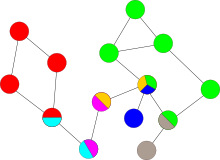
\includegraphics[]{imgs/bicomp.png}
    \end{center}
    Construct a tree of bi-connected components of the graph.
    Some of the approaches related to this structure needs you to do some updates in the parent of the node.

    The application is a problem with a lot of queries
    each query will give 3 vertices a b and c and ask if there is a path that goes from a to b, without passing in c.
    The answer is no if a ==b, a == c or c is an articulation point and is in the path of the block cut tree going from a to b.
    \lstinputlisting{./solutions/Graph/block_cut_tree.cpp}

    \subsection{Two Edge Connected Components}
    Decompose the graph in Components connected by at least two edges.
    Can be used to create a tree as well. a "block cut" decomposition, but with edges instead of vertices.

    \lstinputlisting{./solutions/Graph/2cc.cpp}

    

    